\documentclass[a4paper,11pt]{report}

%%%% PREAMBLE
\usepackage{pdfpages}
\usepackage{scrextend}
\setlength\parindent{12pt}
\usepackage{graphicx}
\usepackage{subfig}
\usepackage{float}
\usepackage{relsize}
\usepackage{amsmath}
\usepackage{amssymb}
\usepackage{textcomp}
\usepackage{hyperref}
\usepackage{lscape}
\usepackage{longtable}
\usepackage{gensymb}
\hypersetup{
    colorlinks=true,
    linkcolor=blue,
    filecolor=magenta,      
    urlcolor=cyan,
}

%\usepackage[margin=1.0in]{geometry}

%%%%  Add some length to the page, as margins always seem too big.  
\addtolength{\topmargin}{-1.5in}
\addtolength{\textheight}{2in}

\begin{document}

%%%%  Number the initial front matter with roman numerals
\pagenumbering{roman}


%%%%  TITLE PAGE
%%  Here are the elements that make up the title page of the document.  

\thispagestyle{empty}  %%  Make the title page have no number.  

%%%%  INSERT TITLE AND NAME HERE!!
\title{\LARGE
Creating a Geospatial Macro Level Feature Database}

\author{Jason Brewer
\\    \\    \\
Final Report
\\    \\
Submitted to 
\\    \\    \\ 
The University of Liverpool
\\    \\
\\    \\
in partial fulfilment of the requirements
\\
for the degree of 
\\     \\
MASTER OF SCIENCE
\\     \\    \\    \\
}


%%  Fill in a date here if you want, or comment out the line below and
%%  the current date will be automatically inserted for you.  
\date{\today}


\maketitle

\newpage

%%%%  TABLE OF CONTENTS  
%%%%      Usually the following command will give you the formatting you want.  

\tableofcontents

%% declaration of whatever is not needed in this document

%%%%  LIST OF FIGURES
%%%%      Comment out this line if you have no figures in your document.  
%\listoffigures


%%%%  LIST OF TABLES  
%%%%      Comment out this next line if you have no tables in your document.  
%\listoftables


\newpage

%%%%  Turn page numbering back to arabic.  This also resets the numbering
%%%%  to begin again at page 1.  

\pagenumbering{arabic}

%%%%  INTRODUCTION

\chapter{Problem Summary}\label{chap:summary}

Blind or visually impaired (BoVI) individuals face many day to day issues regarding the ability to navigate the outdoor world with confidence. As highlighted by Quinonoes et al. \cite{quinones_supporting_2011}, a given hardware and software system for BoVI users must address navigation focussing on recovery from mistakes on a given route, losing one's way, unfamiliar routes and changes to a route which the system must react to efficiently and robustly. 

By understanding the needs of the BoVI user, it becomes apparent that a system must be able to identify meaningful waypoints on a given outdoor route whilst at the same time not supplying an overwhelming amount of information. In effect, the system must act like a background process with an occasional element of interactivity: gathering useful information about the world as it would be perceived by a sighted person and, when required, relaying relevant information back to the BoVI user when required. 

The system previously proposed to tackle this problem, known as Siloam, is comprised of four software components:

\begin{itemize}
	\item SiloamSee (the data collection subsystem)
	\item SiloamLearn (the machine learning subsystem)
	\item SiloamSilo (the online data storage subsystem)
	\item SiloamRoute (the navigation subsystem)
\end{itemize}

Together these components aim to define a standard whereby the information of street level macro level features can be collected and analysed in any arbitrary location. 

The project is being developed in conjunction with another University of Liverpool student. It is they who will deal with the development of SiloamRoute. Because of this and issues that will be covered in chapter \ref{chap:evaluation}, only details of the development of SiloamSee and SiloamLearn will be explored in this document.       

\chapter{Outputs}\label{chap:outputs}

\section{SiloamSee}\label{sec:SS}

The original plan for the SiloamSee component, as discussed in section 2.2.3 of the proposed design and specification, was to extend the open source stock Android camera application from the KitKat version of the operating system. This was the last to feature so called ``photo sphere'' functionality as standard: that is, the ability to capture a 360\degree{}  panoramic spherical image. This is represented in two dimensions in an equirectangular Plate Carr�e projection, which is how the photo sphere is stored on any given device. The proposed extension would utilise aspects of the Google Project Tango C++ API \cite{noauthor_tango_nodate} to include the collection of depth information whilst encoding the RGB data captured by the device that has been used to test the final implementation of SiloamSee, the Lenovo Phab 2 Pro (henceforth referred to as ``P2P''). 

However, this approach proved unsuitable because most of the Android source would need to be built along with the stock camera application resulting in a non modular result. Efforts were made to extend the open source Android application Focal \cite{xplodwild_android_packages_apps_focal:_2017} which also features photo sphere functionality. These efforts also proved fruitless both because of the target device of the application, the LG Nexus 4, and the lack of active development, the last commit being on 20/02/2014. The application built and ran on the P2P but was too unstable.

A more actively developed open source application is Matthieu Labb\`e's RTAB-Map \cite{noauthor_rtabmap:_2017}. A design choice was made to move away from the photo sphere plus depth information idea and focus on the full 3D model capturing that RTAB-Map offers natively. Labb\`e's creation was extended to include GPS and magnetometer data which is shown in figure \ref{fig:SSActivity}. Primarily using Java, three extra buttons were added to the main activity of the application (GET HEADING, START GPS and STOP GPS) as well as real time updates of the last GPS coordinate captured by the P2P. The core of RTAB-Map and these subtle extensions form the SiloamSee subsystem.

As soon as the application starts, the GPS sensors are polled at a minimum of two second intervals. The actual interval can be larger that this due to the nature of the Android GPS polling method and various multithreading behaviours inherent in most modern operating systems. When the user has finished capturing the current outdoor location with SiloamSee, it is recommended the press the STOP GPS button to ensure the OBJ 3D model file export, another feature included as standard in RTAB-Map, executes without error. 

\begin{figure}[H]
\centering
	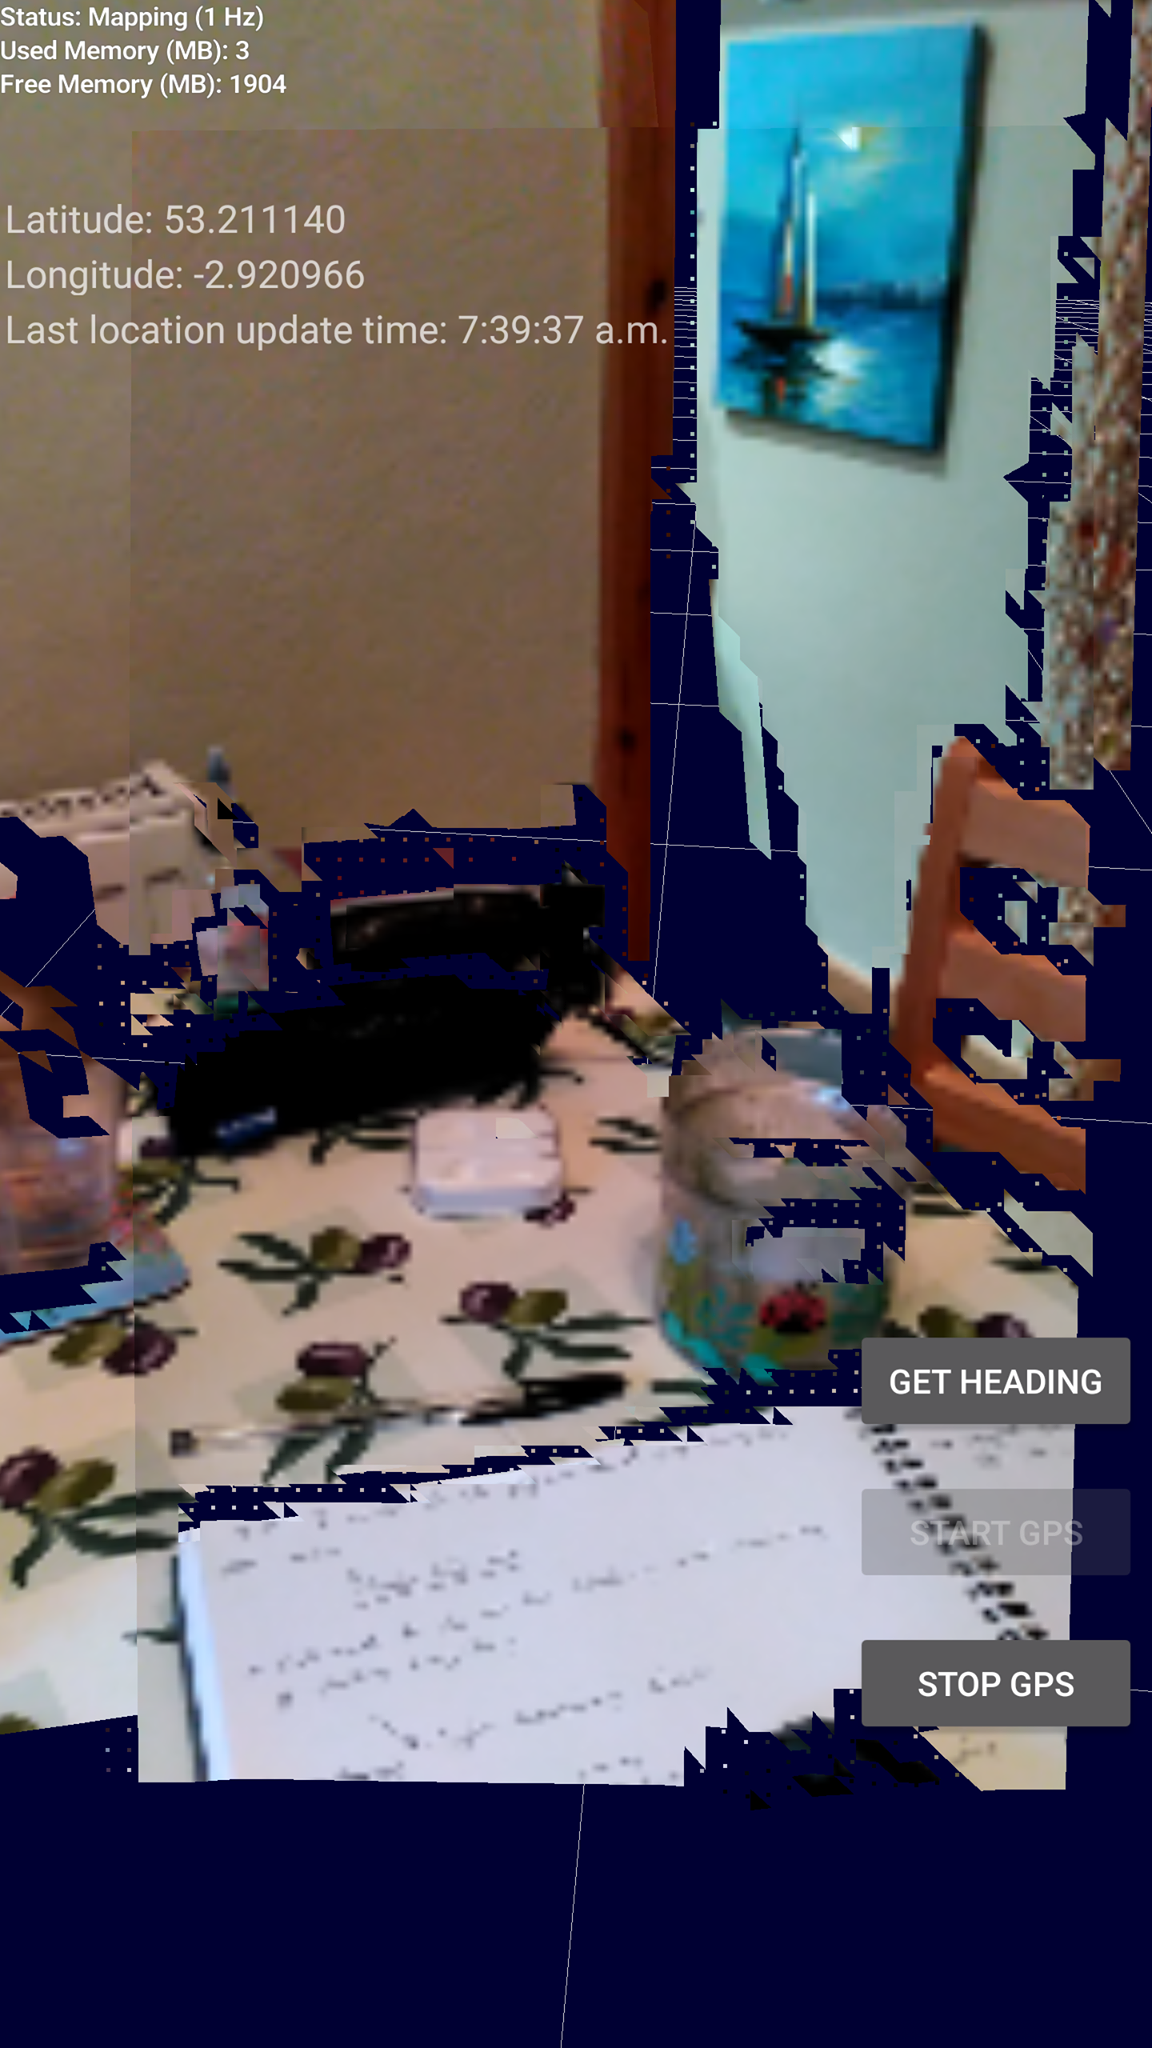
\includegraphics[scale=0.15]{SSScreenshot}
	\caption{Sample view of the extended RTABMapActivity that forms the basis of the SiloamSee Android application}
	\label{fig:SSActivity}
\end{figure}

\begin{figure}[H]
\centering
	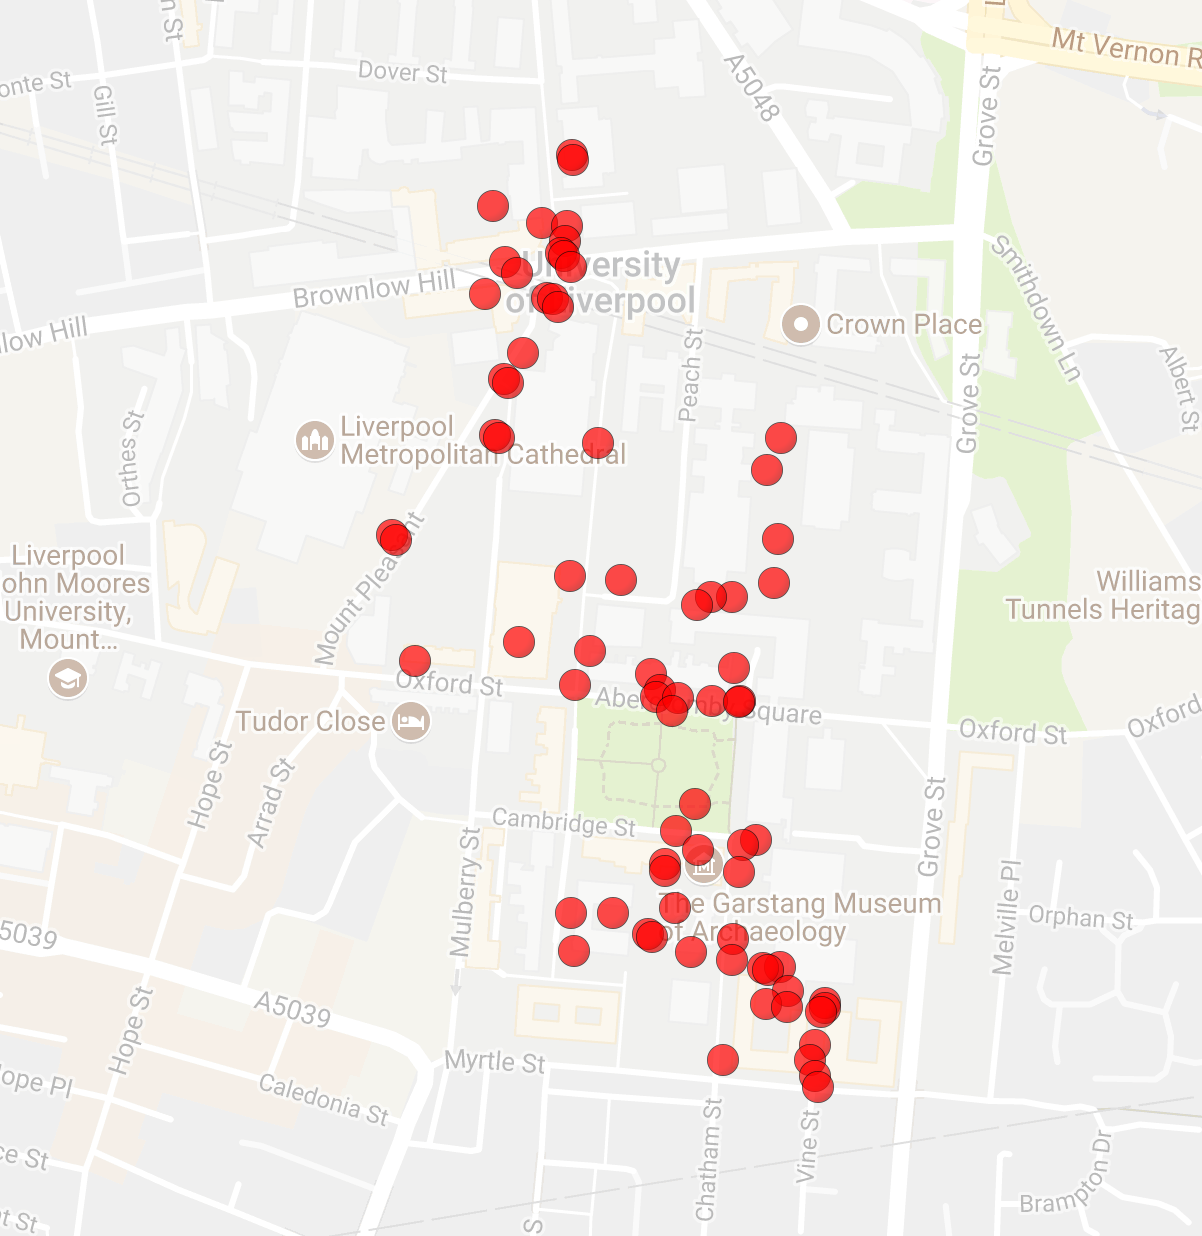
\includegraphics[scale=0.4]{mapping}
	\caption{Map showing the locations of the 76 locations captured by SiloamSee}
	\label{fig:mapping}
\end{figure}

The locations of the 76 models captured by a P2P running SiloamSee are showed in figure \ref{fig:mapping}. Each model was then labelled as either test, train or ground truth data to correspond to the areas shown in figure 2.6 of the proposed design and specification. 

\section{Data Preparation}\label{sec:dataPrep}

Taking inspiration from the methods presented by Fehr et al. \cite{fehr_covariance_2016} , the next step in development was to generate an RGB-D dataset from the 3D models generated by SiloamSee. The paper discusses using not just RGB and depth images (``D'' images) but also RGB representations of the surface normals (``N'' images) of a given 3D scene, the grayscale images (``I'' images) and various applications of the Sobel filter. 

With its powerful Python scripting interface, the open source 3D modelling application Blender \cite{foundation_blender.org_nodate} was a good candidate to render RGB/D/I/N representations of a variety of views of the the 76 models captured by SiloamSee. To this end a script, Blender\_ImportAndRender.py, was produced that contains functions to automatically import and render the RGB/D/I/N data for 16 views of each of the 76 models, totalling to 4864 2D images in total. The placement of the cameras that were produced by the script are shown in figure \ref{fig:blenderCams}. 

\begin{figure}[H]
\centering
	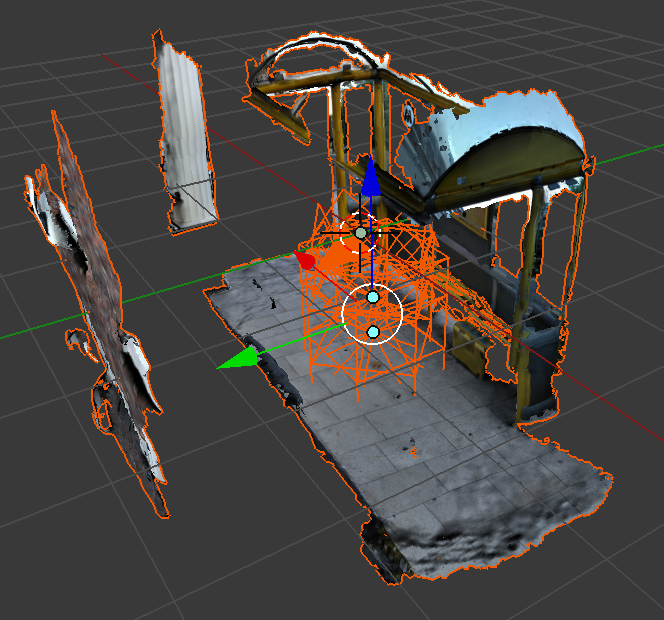
\includegraphics[scale=0.4]{blenderCams}
	\caption{Sample bus stop model. The orange mass centred around the axis representation in the centre of the image is the 16 cameras. They face outwards away from the central point. Each are offset 45\degree{} from eachother to ensure correct overlapping so no macro level features will be lost}
	\label{fig:blenderCams}
\end{figure}

The project also makes use of 3D models downloaded from the Trimble Warehouse \cite{trimble_inc._3d_nodate} to better train the support vector machine (SVM) in the SiloamLearn subsystem. Therefore, Blender\_ImportAndRender.py also features functionality to define a square/rectangular perimeter of cameras around an imported DAE 3D model. This is shown in figure \ref{fig:blenderCamsInteractive}. RGB/D/I/N representations are also generated for these imported models.

\begin{figure}[H]
\centering
	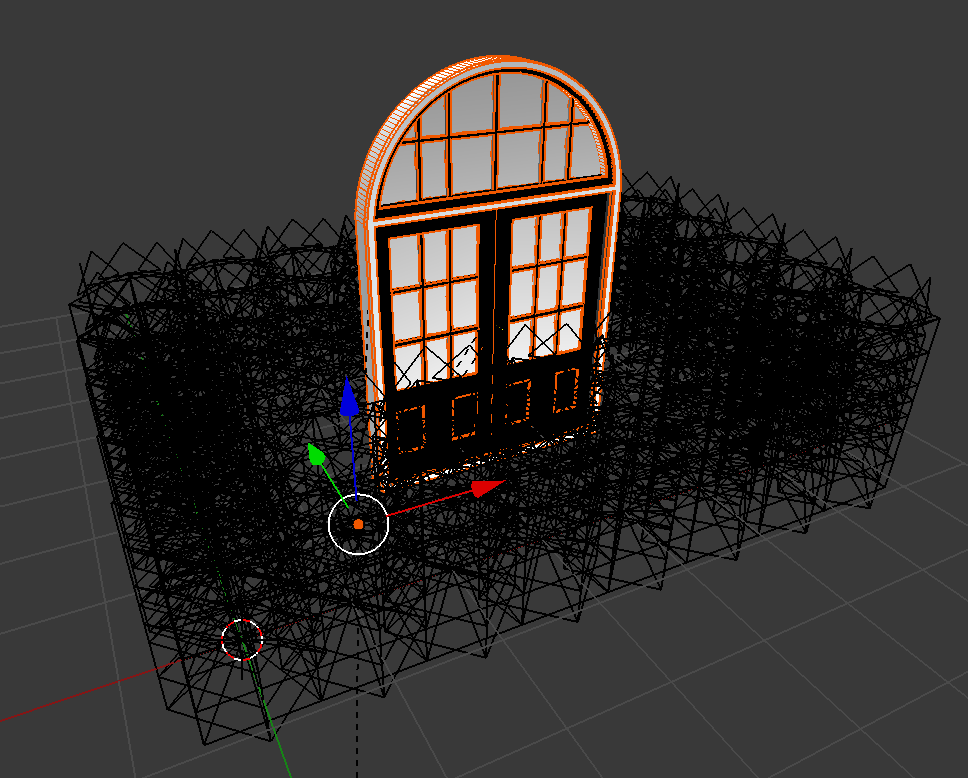
\includegraphics[scale=0.3]{blenderCamsInteractive}
	\caption{The model here is the so-called ``ArchDoor''. It is surrounded by a rectangular structure of pillars of cameras of dimension 7 units by 4 units. In an interactive fashion, after the user has imported the model and specified the dimensions of the camera rig, the imported model is selected so that it can be moved into the centre of the rig}
	\label{fig:blenderCamsInteractive}
\end{figure}

\section{SiloamLearn}\label{sec:SL}

Again following the methods of Fehr et al. \cite{fehr_covariance_2016}, the SiloamLearn C++ application developed thus far creates a database of all of the paths to the 4864 images produced by Blender\_ImportAndRender.py and uses the DBSCAN \cite{ester1996density} algorithm to segment the objects of interest from the floor plane. The abstract version of this algorithm can be condensed as follows:

\begin{itemize}
	\item 1. Process the bottom quarter of an N image to get an idea of possible RGB values of floor normals
	\item 2. Process the rest of the image and find all pixels that fall within the range of RGB values found in step 1. Use this to create a ``floor estimation'' pixel set
	\item 3. Remove all the pixels in the ``floor estimation'' set from the D image
	\item 4. Run the DBSCAN algorithm and add all pixels in clusters of less than size ``kNormalNoiseThreshold'' (experimentally set at 2000) to the ``floor estimation'' set
	\item 5. Make all the pixels in the ``floor estimation'' set black for each of the RGB/D/I/N images
\end{itemize}

The implementation of DBSCAN is provided by the pyclustering C++ library  \cite{noauthor_annoviko/pyclustering:_nodate}. A graphical representation and a sample result is show in figure \ref{fig:dbscan}.

\begin{figure}[H]
\centering
	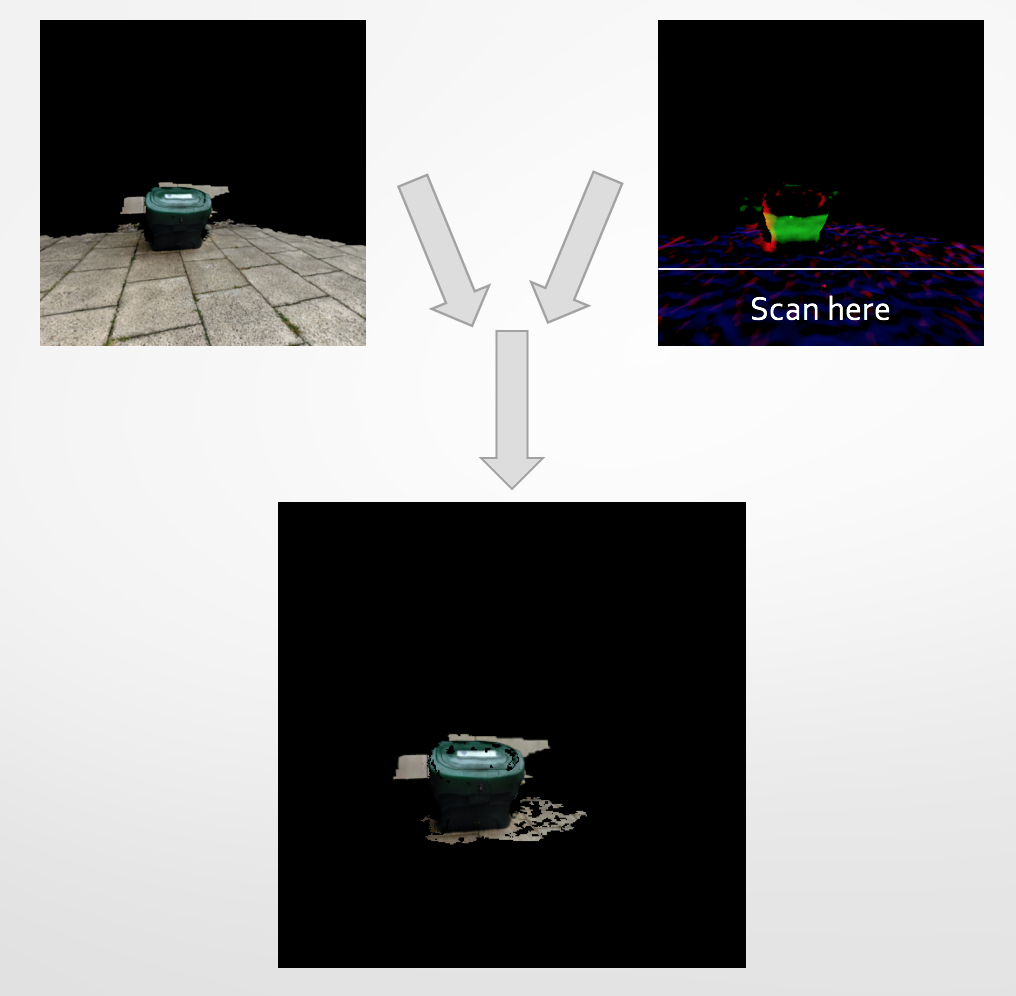
\includegraphics[scale=0.5]{dbscan}
	\caption{Sample results of the experimental floor removal algorithm}
	\label{fig:dbscan}
\end{figure}

It is important to mention that development of SiloamLearn is still ongoing. Currently in development is the generation of various applications of the Sobel filter to I and D images to complete the dataset needed to form the covariance descriptors used to train the SVM outlined in Fehr et al. \cite{fehr_covariance_2016}. The final application will use the trusted Sobel functionality from OpenCV \cite{noauthor_opencv_nodate}.

\chapter{Evaluation}\label{chap:evaluation} 

Although a working Android application has been completed, initial teething difficulties with the development of SiloamSee meant that in reality development took four weeks instead of one, as shown by the arrow extending from the allotted time in figure \ref{fig:failures}. The light gray circle shows the actual completion date. Following this, development of SiloamLearn started 3 weeks late and continues to the day of writing. This means that, while essentially a simple text processing task, the interface between SiloamLearn and SiloamSilo has yet to begin. Having said that the library needed, cpprestsdk \cite{noauthor_cpprestsdk:_2017}, is in place and is well maintained and tested. 

Furthermore, while figure \ref{fig:dbscan} shows a fairly successful application of the experimental floor removal algorithm this is not the case for all images tested. In some cases very few areas of the floor plane are removed and in other cases large parts of the objects of interest in the image are removed. At present it is not a general solution; further experimentation with ``kNormalNoiseThreshold'' as well as the parameters of DBSCAN, $\epsilon$ and minPts is required.

While too late in the day to change the course of the project completely, future development may make use of PCL \cite{noauthor_pcl_nodate} to process coloured point clouds instead of RGB-D data. 3D OBJ files are readily converted to point clouds using the library and may lead to greater insights into the data captured by SiloamSee. 

\begin{figure}[h]
\centering
	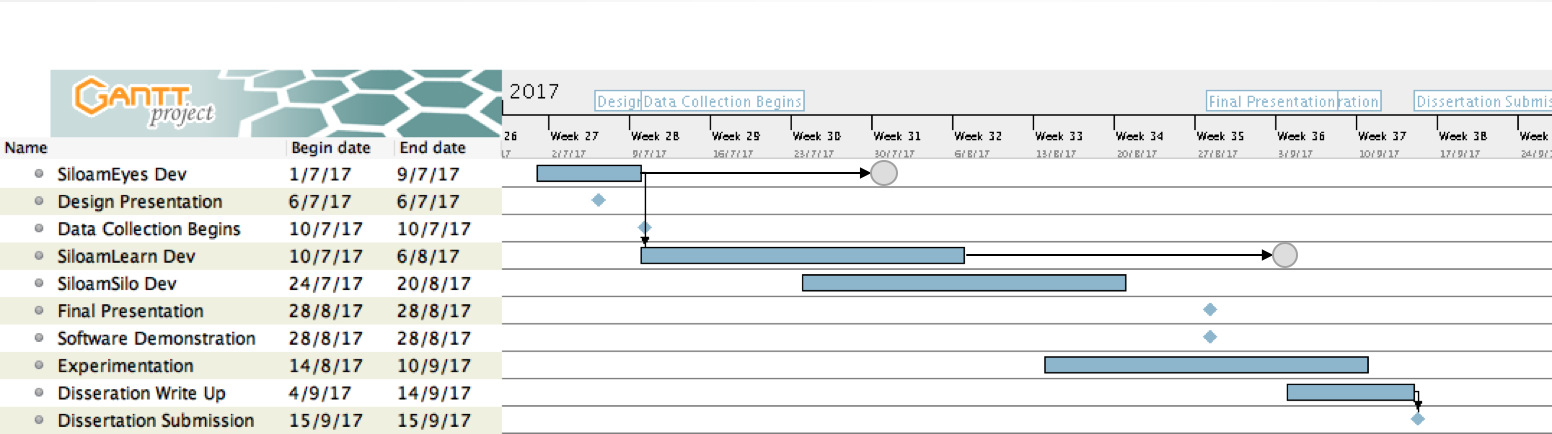
\includegraphics[scale=0.5]{amendedGantt}
	\caption{The original gantt chart from the proposed design and specification with indications of actual development timescales. The light gray circle in the first row signifies the real completion date while the light gray circle in the SiloamLearnDev row corresponds to the present day}
	\label{fig:failures}
\end{figure}

\bibliographystyle{IEEEtran}
\bibliography{References}

\end{document}
